
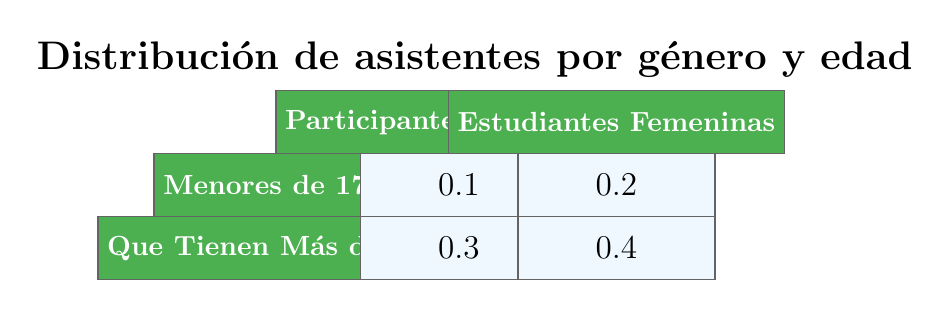
\begin{tikzpicture}[scale=0.8]
  % Definir colores
  \definecolor{headercolor}{RGB}{76, 175, 80}
  \definecolor{cellcolor}{RGB}{240, 248, 255}
  \definecolor{bordercolor}{RGB}{100, 100, 100}

  % Configurar estilo de nodos
  \tikzset{
    header/.style={fill=headercolor, text=white, font=\bfseries, minimum height=0.8cm, minimum width=2.5cm, draw=bordercolor, line width=0.5pt},
    cell/.style={fill=cellcolor, minimum height=0.8cm, minimum width=2.5cm, draw=bordercolor, line width=0.5pt, font=\large},
    label/.style={font=\bfseries, minimum height=0.8cm, minimum width=2.5cm}
  }

  % Encabezados de columnas
  \node[header] at (2.5, 2) {Participantes Masculinos};
  \node[header] at (5, 2) {Estudiantes Femeninas};

  % Etiquetas de filas
  \node[header] at (0, 1) {Menores de 17 años};
  \node[header] at (0, 0) {Que Tienen Más de 17 años};

  % Celdas de datos
  \node[cell] at (2.5, 1) {0.1};
  \node[cell] at (5, 1) {0.2};
  \node[cell] at (2.5, 0) {0.3};
  \node[cell] at (5, 0) {0.4};

  % Título de la tabla
  \node[label, font=\Large\bfseries] at (2.75, 3) {Distribución de asistentes por género y edad};
\end{tikzpicture}

